\begin{definition}[Posto de uma transformação linear]
  O \textbf{posto} de uma transformação linear $T:\mathbb{R}^{m}\to\mathbb{R}^{n}$ é definido por $\posto(T)=\dim(\Img T)$.\\
  Isto é, o número máximo de vetores linearmente independente entre $Te_1,\cdots,Te_m$.\\
  Ou, equivalentemente o numero máximo de columas linearmente independente da matriz $T$.
\end{definition}
\begin{note}
  Este tambem é o número máximo de linhas linearmente independentes dessa matriz e que o posto de $T$ é igual a $r$ se, somente se, a matriz $T$ comtem um determinante menor $r\times r$ não nulo, mas qualquer determinante menor de ordem $r+1$ é zero. 
\end{note}
\begin{definition}[Posto de uma aplicação diferenciável]
  Seja $f:U\subseteq \mathbb{R}^{m}\to\mathbb{R}^{n}$ diferenciável no ponto $x\in U$, definimos \text{posto} de $f$ em $x$ dado por $\posto f=\posto f^{\prime}(x)$. 
\end{definition}
\begin{note}
  \phantom{xxx}
  \begin{itemize}
    \item $\posto f\leq\min\{m,n\}$.
    \item Uma inmersão $f:u\to\mathbb{R}^{n}$ diferenciável no aberto $U\subseteq\mathbb{R}^{m}$ tem posto $m$ em todos os pontos $x\in U$.
    \item Uma submersão $f:U\to\mathbb{R}^{n}$ tem posto $n$ com qualquer ponto. 
  \end{itemize}
\end{note}
\begin{example}
  Seja $f:U\subseteq\mathbb{R}^{m}\to\mathbb{R}^{n}$ uma aplicação diferenciável.
  \begin{enumerate}
    \item Suponha $n=1$.\\
      A derivada $f^{\prime}(a)$ e a matriz $1\times m$.\\
      $$f^{\prime}(a)=\left( \frac{\partial f}{\partial x_1}(a),\cdots,\frac{\partial f}{\partial x_m}(a) \right).$$
      O posto de uma matriz pode ser
      \begin{itemize}
        \item $1$, sempre que $a$ é ponto regular.
        \item $0$, sempre que $a$ é ponto crítico. 
      \end{itemize}
    \item $m=n=2$.\\
      Suponha $f$ holomorfa (isto é, que $f=u+iv$ onde $u_{x}=v_{y}$ e $u_{y}=-v_{x}$ que são as equações de Cauchy-Riemman.)\\
      \textbf{Afirmação:} O posto de $f^{\prime}(z)$ é $0$ ou $2$.
      \begin{align*}
        Jf(z)\begin{pmatrix}
          u_{x}(z) & u_{y}(z) \\
          -u_{y}(z) & u_{x}(z)
        \end{pmatrix}.
      \end{align*}
      Logo, $\det(Jf(a))=u_{x}^{2}(z)+u_{y}^{2}(z)=0$ se, somente se, $u_{x}=u_{y}=0$, logo $Jf(a)=0$, assim o $\posto f^{\prime}(z)=0$.\\
      Caso contrario, $\det(Jf(a))\geq 0$, então $\posto f^{\prime}
      (z)=2$, ja que $Jf(a)$ é invertível.
    \item $m=n=2$.\\
      Suponha $f$ dada por $f(x,y)=(x^{3},x^{2})$, note que
      \begin{align*}
        Jf(x,y)=\begin{pmatrix}
          3x^{2} & 0 \\
          0 & 2y
        \end{pmatrix}.
      \end{align*}
      \begin{itemize}
        \item Se $x\neq 0$ e $y\neq 0$, $Jf(x,y)$ é invertível, logo posto $Jf(x,y)=2$.
        \item Se $(x,0)$ com $x\neq 0$ ou $(0,y)$ com $y\neq 0$, o posto é $1$.
        \item Se $x=y=0$, posto é zero.
      \end{itemize}
  \end{enumerate}
\end{example}
\begin{proposition}
  Se $f:U\subseteq\mathbb{R}^{m}\to\mathbb{R}^{n}$ é $C^{1}$ e o $\posto f^{\prime}(a)=r$, com $a\in U$, então existe uma vizinhança $B$ de $a$ contínua em $U$ tal que o posto de $f^{\prime}(x)\geq r$ para todo $x\in B$ 
\end{proposition}
\begin{proof} 
  Sabemos que $\posto f^{\prime}(a)=r$. Isto é, que existe um determinante menor $r\times r$ da matriz $Jf(a)$ não nulo que é diferente de zero. Assim, pela continuidade do $f^{\prime}(a)$ temos que este mesmo menor é não nulo em todos os pontos de uma vizinhança $B$ de $a$. Logo, $\posto f^{\prime}(x)\geq r$, com $x\in B$. 
\end{proof}
Agora, uma questão, dada uma aplicação $f$ com posto constante o que podems dizer sobre sua forma local?\\
Resposta: Localmente, a menos de mudanças de coordenadas (difeomorfismos), $f$ se comporta como uma projeção.
\begin{definition}
  Dada uma descomposição $\mathbb{R}^{m+n}=\mathbb{R}^{m}\oplus\mathbb{R}^{n}$ diremos que um conjunto $X\subseteq \mathbb{R}^{m+n}$ é verticalmente convexo quando todo segmento vertical $[(x,y^{\prime}),(x,y^{\prime\prime})]$ cujas extremidades pertenecen a $X$, esta contido em $X$.
  \begin{center}
    \begin{tikzpicture}[scale=1.2]
  \draw[->] (-1,0) -- (4,0) node[right] {$\mathbb{R}^m$};
  \draw[->] (0,-1) -- (0,3) node[above] {$\mathbb{R}^n$};
  \draw (1,-1) -- (1,3);
  \draw (3,-1) -- (3,3);

  \fill (1,0) circle (2pt);
  \node[below] at (1.2,0) {$x$};

  \fill (1,1) circle (2pt);
  \node[right] at (1,1) {$(x,y^{\prime})$};

  \fill (1,3) circle (2pt);
  \node[right] at (1,3) {$(x,y^{\prime\prime})$};

  \fill (3,0) circle (2pt);
  \node[below] at (3.2,0) {$w$};

  \fill (3,1) circle (2pt);
  \node[right] at (3,1) {$(w,y^{\prime})$};

  \fill (3,3) circle (2pt);
  \node[right] at (3,3) {$(w,y^{\prime\prime})$};

\end{tikzpicture}
  
  \end{center}
\end{definition}
\begin{example}
  Seja $X=V\times W$.\\
  \begin{itemize}
    \item $V\subseteq\mathbb{R}^{m}$ qualquer.
    \item $W\subseteq \mathbb{R}^{n}$ é convexo. 
  \end{itemize}
  Então $X$ é verticalmente convexo. 
\end{example}
\begin{lemma}\label{lema:3.11-1teoremadoposto}
  Seja $U\subseteq \mathbb{R}^{m+n}=\mathbb{R}^{m}\oplus\mathbb{R}^{n}$ um aberto verticalmente convexo.\\
  Se $F:U\to\mathbb{R}^{p}$, possui $\partial_{2}f=0$ em $U$, então $f$ não depende da segunda variável, i.é, $f(x,y_1)=f(x,y_2)$ para todo $y_1,y_2\in\mathbb{R}^{n}$. 
\end{lemma}
\begin{proof} 
  Dados $(x,y_1),(x,y_2)\in U$, defina o caminho $\lambda:[0,1]\to\mathbb{R}^{p}$ dada por $\lambda(t)=f(x,y_1+t(y_2-y_1))$ para todo $t\in[0,1]$, temos
  \begin{align*}
    \lambda^{\prime}(t)=f^{\prime}(x,y_1+t(y_2-y_1))\cdot (y_2-y_1)=0
  \end{align*}
  Logo $\lambda$ é constante, em particular $\lambda(0)=\lambda(1)$, ou seja $f(x,y_1)=f(x,y_2)$. 
\end{proof}
\begin{lemma}\label{lema:3.11-2teoremadoposto}
  Seja $E\subseteq\mathbb{R}^{m+p}$ um espaço vetorial de dimensão $m$. Então existe uma decomposição em soma direta $\mathbb{R}^{m+p}=\mathbb{R}^{m}\oplus\mathbb{R}^{p}$ tal que a primeira projeção $\pi:\mathbb{R}^{m+n}\to\mathbb{R}^{m}$ dada por $\pi(x,y)=x$ aplica $E$ isomorficamente sobre $\mathbb{R}^{m}$. 
\end{lemma}
\begin{proof} 
  Sabemos que $\dim(E)=m$, escolha uma base $\{e_1,e_2,\cdots,e_m\}\subseteq \mathbb{R}^{m+p}$ e defina a matriz $A$ como a matriz dada por columas $A=(e_1,e_2,\cdots,e_m)$, note que $A$ é uma matriz $(m+p)\times m$.\\
  Note que pela construção $A$ tem posto $m$. Portanto, existe um comjunto de $m$ linhas da matriz que são linearmente independentes. Sejam os indices dessas linhas $i_1\leq i_2\leq \cdots \leq i_m$ onde $i_k\in\{1,\cdots,m+p\}$.\\
  Definamos a projeção $\pi:\mathbb{R}^{m+p}\to\mathbb{R}^{m}$ dada por $\pi(x)\to (x_{i_1},x_{i_2},\cdots,x_{i_m})$. Note que em termos matriciais $\pi$ é representada por uma matriz $m\times (m+p)$ que tem $1$ nas posições $(k,i_k)$ e $0$ nas demais (troca linhas).\\
  Aplique $\pi$ a cada columa $e_j$ de $A$. Observe que o resultado $\pi(e_j)$ é um vetor no $\mathbb{R}^{m}$ formado pelas coordenadas $j_1,j_2,\cdots,j_m$ de $e_j$. Assim, construa a matriz $B$ como la matriz dada por columas $B=\left( \pi(e_1),\pi(e_2),\cdots,\pi(e_m) \right)$ e note que $B$ é uma matriz $m\times m$ com $\posto B=m$. Portanto, $B$ é invertível e $\det(B)\neq 0$.\\
  \textbf{Afirmação:}$\pi\big|{E}$ é isomorfismo \textcolor{red}{Verificar!}\\
  Agora, complete as $m$ coordenadas escolhidas $(i_1,i_2,\cdots,i_m)$ com as $p$ coordenadas restantes. Reordene as coordenadas de $\mathbb{R}^{m+p}$ de modo que
  \begin{itemize}
    \item As primeras $m$ coordenadas sejam exatamente $x_{i_1},x_{i_2},\cdots,x_{i_m}$.
    \item As últimas $p$ coordenadas sejam as demais. 
  \end{itemize}
  Nessa nova reordenação $\pi(u,v)=u$ para todo $u\in\mathbb{R}^{m}$ e $v\in\mathbb{R}^{p}$ com $E$ sendo isomorfo a $\mathbb{R}^{m}$ vía $\pi$, i.é, existe $T$ transformação linear tal que $E=\{(u,Tu):u\in\mathbb{R}^{m}\}$ o gráfico de $T$.\\
  Assim, $\mathbb{R}^{m+p}=\mathbb{R}^{m}\oplus\mathbb{R}^{p}$ com $\pi\big|_{E}$ isomorfismo. 
\end{proof}
\begin{theorem}[Teorema do posto]
  Seja $f:U\subseteq\mathbb{R}^{m+n}\to\mathbb{R}^{m+p}$ de classe $C^{1}$ ($k\geq 1$) com posto constante igual a $c$ em todos os pontos do aberto $U$. Então para cada $a\in U$ existem
  \begin{itemize}
    \item Um $C^{k}$-difeomorfismo $\alpha$ de um aberto de $\mathbb{R}^{m}\times\mathbb{R}^{n}$ sobre uma vizinhança de $a$.
    \item Um $C^{k}$-difeomorfismo $\beta$ de uma vizinhança de $f(a)$ sobre um aberto de $\mathbb{R}^{m}\times\mathbb{R}^{p}$. 
  \end{itemize}
  Tais que $(\beta\circ f\circ \alpha)(x,y)=(x,0)$.
  \begin{center}
    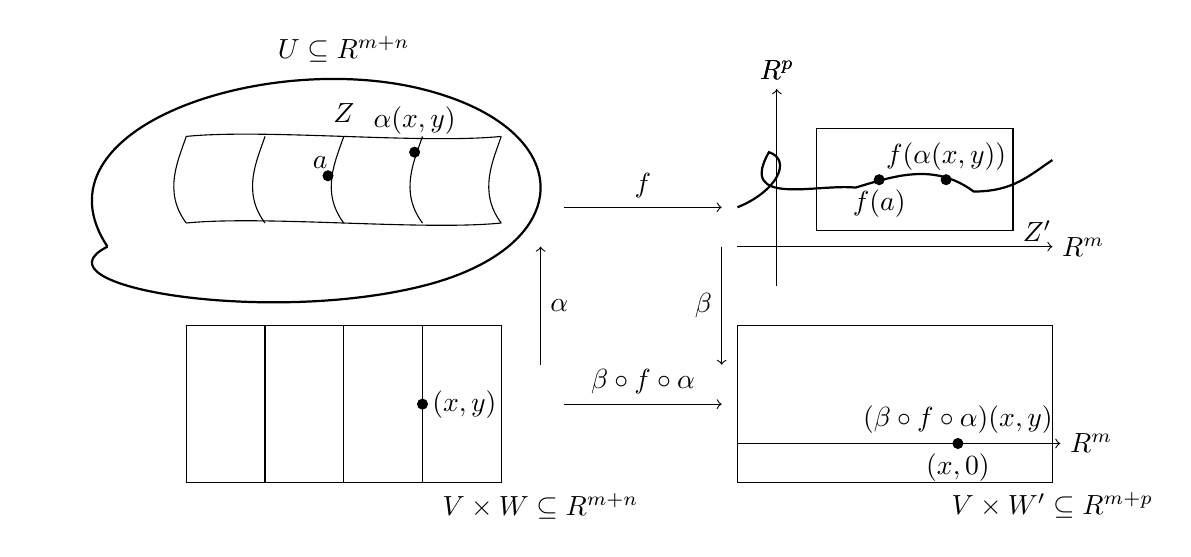
\begin{tikzpicture}[scale=1]

% ======================
% REGIÓN SUPERIOR (U)
% ======================

% Contorno tipo "orgánico"
\draw[thick] (-7,1.5) .. controls (-8,3) and (-5,4) .. (-3,3.5)
             .. controls (-1,3) and (-1,1.5) .. (-3,1)
             .. controls (-5,0.5) and (-8,1) .. (-7,1.5);

\node at (-4,4) {$U\subseteq \mathbb{R}^{m+n}$};
\node at (-4,3.2) {$Z$};

% "Fibras" (curvas horizontales suaves)
\foreach \y in {1.8,2.9} {
    \draw (-6,\y)
    .. controls (-5,{\y+0.1}) and (-3,{\y-0.1}) ..
    (-2,\y);
}

% Líneas verticales (estructura tipo producto)
\draw (-5,1.8)
.. controls (-5.3,2.2) and (-5.1,2.6) ..
(-5,2.9);

\draw (-4,1.8)
.. controls (-4.3,2.2) and (-4.1,2.6) ..
(-4,2.9);

\draw (-3,1.8)
.. controls (-3.3,2.2) and (-3.1,2.6) ..
(-3,2.9);

\draw (-6,1.8)
.. controls (-6.3,2.2) and (-6.1,2.6) ..
(-6,2.9);

\draw (-2,1.8)
.. controls (-2.3,2.2) and (-2.1,2.6) ..
(-2,2.9);


% Punto alphaxy
\fill (-3.1,2.7) circle (2pt);
  \node[above] at (-3.1,2.8) {$\alpha(x,y)$};

% Punto a
\fill (-4.2,2.4) circle (2pt);
\node[above] at (-4.3,2.37) {$a$};

% ======================
% REGIÓN INFERIOR (V x W)
% ======================

\draw (-6,-1.5) rectangle (-2,0.5);
\node at (-1.5,-1.8) {$V\times W\subseteq \mathbb{R}^{m+n}$};
% Grid
\foreach \x in {-6,-5,-4,-3,-2} {
    \draw (\x,-1.5) -- (\x,0.5);
}


% Punto (x,y)
\fill (-3,-0.5) circle (2pt);
  \node[right] at (-3,-0.5) {$(x,y)$};

% Flecha h
\draw[->] (-1.5,0) -- (-1.5,1.5);
\node[right] at (-1.5,0.75) {$\alpha$};


% ======================
% LADO DERECHO (R^n)
% ======================

\draw[->] (1.5,1) -- (1.5,3.5);
\node[above] at (1.5,3.5) {$\mathbb{R}^p$};

\draw[->] (1,1.5) -- (5,1.5);
\node[right] at (5,1.5) {$\mathbb{R}^m$};

\fill (2.8,2.35) circle (2pt);
\node[below] at (2.8,2.35) {$f(a)$};

\fill (3.65,2.35) circle (2pt);
\node[above] at (3.65,2.35) {$f(\alpha(x,y))$};

% Rectángulo (W)
\draw (2,1.7) rectangle (4.5,3);
\node[right] at (4.5,1.7) {$Z^{\prime}$};
  
% Curva dentro
\draw[thick] 
  (1,2) 
  .. controls (1.5,2.2) and (1.7,2.6) .. (1.4,2.7)
  .. controls (1,2) and (2,2.3) .. (2.5,2.25)
  .. controls (3,2.4) and (3.5,2.57) .. (4,2.2)
  .. controls (4.5,2.2) and (4.7,2.4) .. (5,2.6);
 
% Flecha f diagonal
\draw[->] (-1.2,2) -- (0.8,2);
\node[above] at (-0.2,2) {$f$};

% Flecha horizontal
\draw[->] (-1.2,-0.5) -- (0.8,-0.5);
\node[above] at (-0.2,-0.5) {$\beta\circ f\circ \alpha$};

% Flecha beta
\draw[->] (0.8,1.5) -- (0.8,0);
\node[left] at (0.8,0.75) {$\beta$};

% Rectangulo final

\draw (1,-1.5) rectangle (5,0.5);
\node[below] at (5,-1.5) {$V\times W^{\prime}\subseteq \mathbb{R}^{m+p}$};

\draw (1.5,1) -- (1.5,3.5);
\node[above] at (1.5,3.5) {$\mathbb{R}^p$};

\draw[->] (1,-1) -- (5.1,-1);
\node[right] at (5.1,-1) {$\mathbb{R}^m$};

\fill (3.8,-1) circle (2pt);
\node[below] at (3.8,-1) {$(x,0)$};
\node[above] at (3.8,-1) {$(\beta\circ f\circ \alpha)(x,y)$};

\end{tikzpicture}
  
  \end{center}
\end{theorem}
\begin{proof} 
  Seja $E=f^{\prime}(a)\left( \mathbb{R}^{m+n} \right)\subseteq \mathbb{R}^{m+p}$. Pelo lema \ref{lema:3.11-2teoremadoposto} existe uma descomposição $\mathbb{R}^{m+p}=\mathbb{R}^{m}\oplus\mathbb{R}^{n}$ tal que a projeção $\pi:\mathbb{R}^{m+p}\to\mathbb{R}^{m}$ restrita a $E$ é isomorfismo. Agora, considere $\pi\circ f:U\to\mathbb{R}^{p}$ y note que $(\pi\circ f)^{\prime}(a)=\pi f^{\prime}(a):\mathbb{R}^{m+n}\to\mathbb{R}^{p}$ é sobrejetica (pois $\pi\big|_{E}$ é isomorfismo).\\
  Logo, pela forma local das submersões existe um difeomorfismo $\alpha\in C^{k}$ e um aberto $V_{0}\times W\subseteq \mathbb{R}^{m}\times\mathbb{R}^{n}$ sobre uma vizinhança aberta de $a$ tal que $(\pi\circ f)\circ \alpha(x,y)=x$. Isto é que $(f\circ \alpha)(x,y)=(x,\lambda(x,y))$ onde $\lambda:V_{0}\times W\subseteq \mathbb{R}^{m}\times\mathbb{R}^{n}\to\mathbb{R}^{p}$ é $C^{k}$.\\
  \textbf{Afirmação:} $\partial_{2}\lambda=0$.\\
  Note que a deriada de $f\circ \alpha$ é
  \begin{align*}
    (f\circ \alpha)^{\prime}(x,y)=\begin{pmatrix}
      I_{\mathbb{R}^{m}} & 0 \\
      \partial_{x}\lambda & \partial_{y}\lambda
    \end{pmatrix}
  \end{align*}
  Sabemos que o $\posto(f\circ\alpha)=\posto(f)=m$, logo $\partial_{y}\lambda=0$.\\
  Então, como $W$ pode ser tomada convexo, pelo lema \ref{lema:3.11-1teoremadoposto} temos que $\lambda(x,y)=\lambda(x,y_0)$.\\
  Agora, considere $\alpha(a_1,a_2)=a$.\\
  Defina a injeção $i:V_{0}\to V_{0}\times W$ dada por $i(x)=(x,a_2)$. Então, obtemos a aplicação $C^{k}$ $h(x)=(f\circ\alpha\circ i)(x)=(x,\alpha(x,a_{2}))$ que tem derivada injetiva em $a_1$, pois
  \begin{align*}
    h^{\prime}(a_1)=\begin{pmatrix}
      I_{\mathbb{R}^{m}} \\
      \partial_{x}\lambda(a_1,a_2)
    \end{pmatrix}.
  \end{align*}
  Do tamanho $p\times m$, logo se $h^{\prime}(a_1)\cdot v=0$ com $v\in\mathbb{R}^{m}$, então $v=0$.\\
  Assim, pela forma local das imersões existe um $C^{k}$ difeomorfismo $\beta$ numa vizinhança de $f(a)$ sobre um aberto de $\mathbb{R}^{m}\times\mathbb{R}^{p}$ tal que $\beta\circ(f\circ\alpha\circ i)(x)=(x,0)$.\\
  Logo, como $f\circ \alpha(x,y)=f\circ\alpha(x,a_2)=f\circ\alpha\circ i(x)$ temos que $(\beta\circ f\circ\alpha)(x,y)=(x,0)$ para todo $y\in W$ e para todo $x$ no aberto $V\subseteq V_{0}\subseteq \mathbb{R}^{m}$, contemdo $a$ e $y$ no $W\subseteq\mathbb{R}^{n}$ 
\end{proof}
\begin{corollary}
  Seja $f:U\subseteq\mathbb{R}^{m}\to\mathbb{R}^{n}$ de classe $C^{1}$ com $U$ aberto, então
  \begin{itemize}
    \item $f$ é localmente injetiva se, somente se é uma imersão.
    \item $f$ é aberta se, somente se, é uma submersão. 
  \end{itemize}
\end{corollary}
